
\section{Results and Analysis}

% \label{sec:main_results}
% Table~\todo{Table X} compares Omni (No-RAG) and RAG-InfiniSST under matched SimulEval settings.
% We report BLEU, StreamLAAL, StreamLAAL\_CA, and \textsc{TermAcc}.
% \todo{Add Table X placeholder.}

\begin{figure*}[t]
\centering
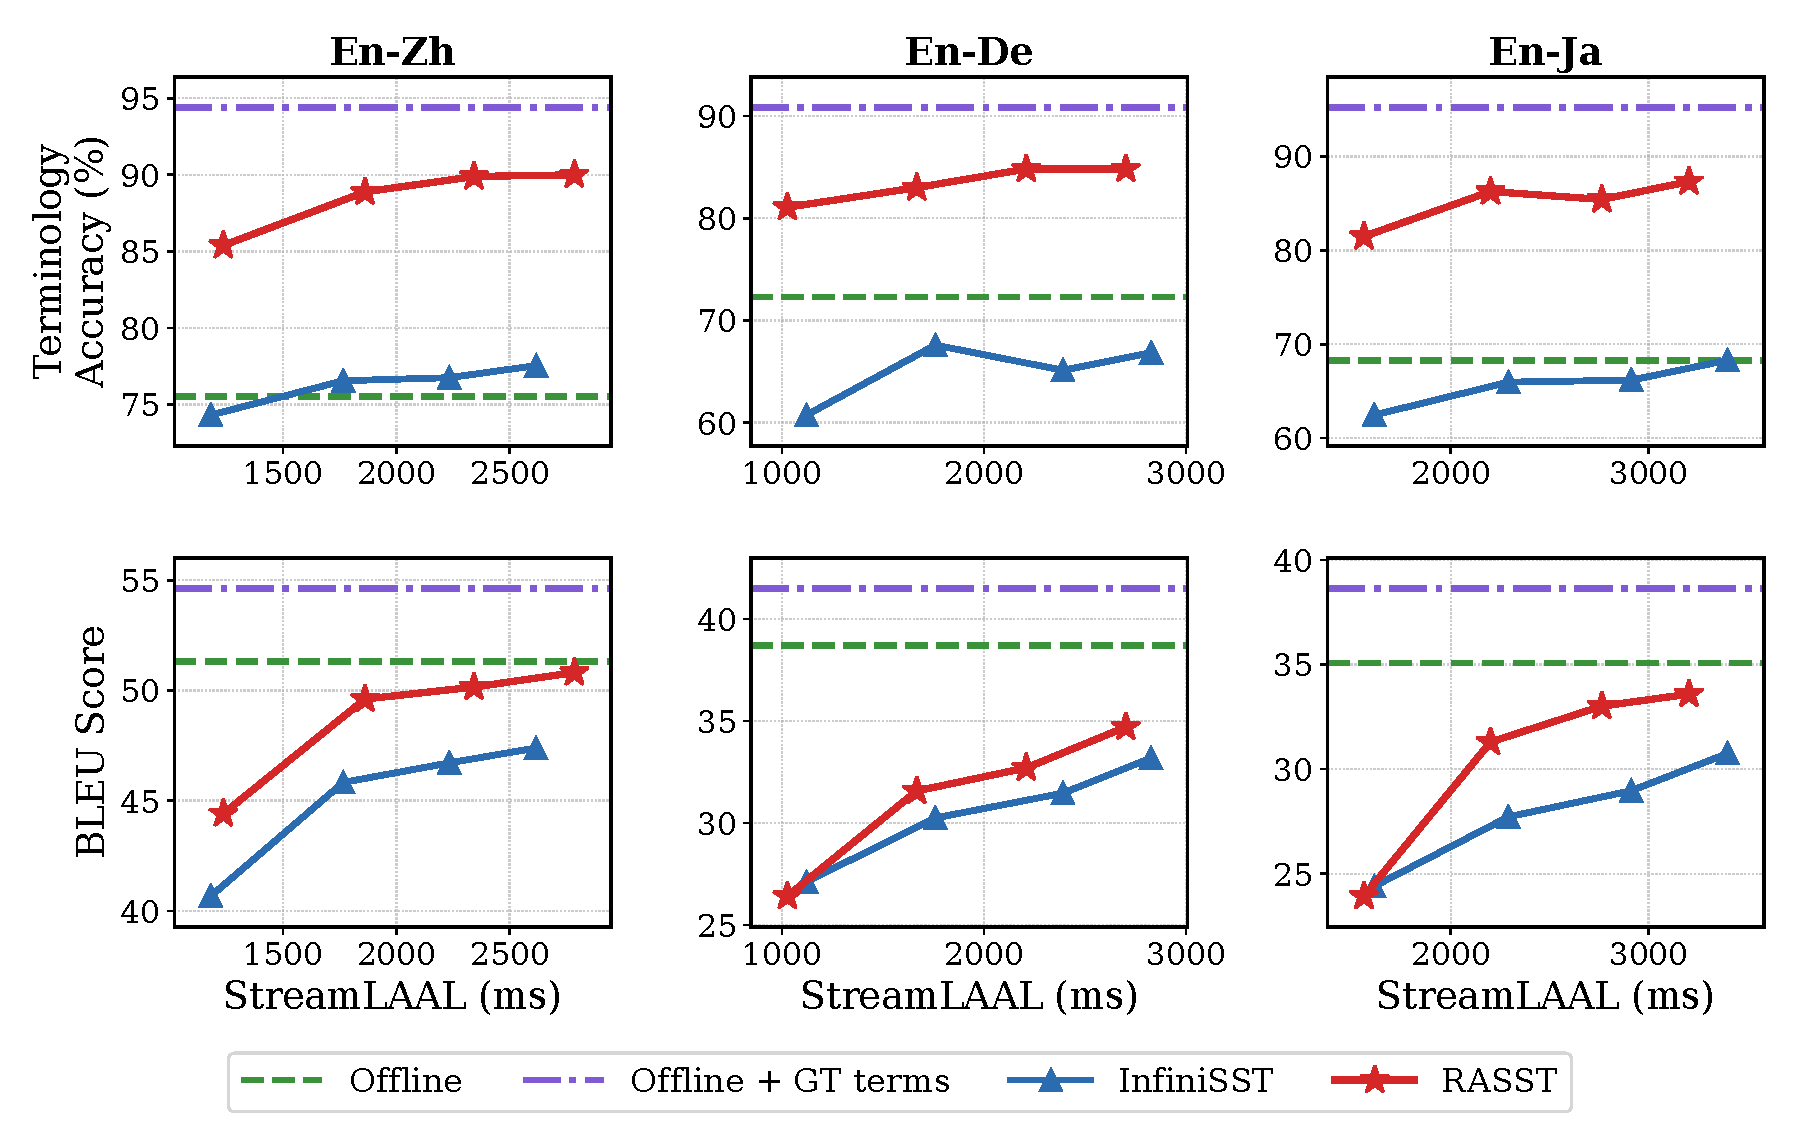
\includegraphics[width=0.9\linewidth]{latex/figures/new_main_result_tagged.pdf}
\caption{Main results on the ACL tagged raw glossary with the final HN1024 retriever at $\tau{=}0.78$. We compare Terminology Accuracy (top) and BLEU (bottom) against StreamLAAL for En-Zh, En-De, and En-Ja. Horizontal lines show full-context offline LLM references, without and with oracle glossary terms. \method improves terminology accuracy over the InfiniSST baseline across all three language directions while maintaining competitive translation quality.}
\label{fig:main_result_1}
\end{figure*}

\begin{figure*}[t]
\centering
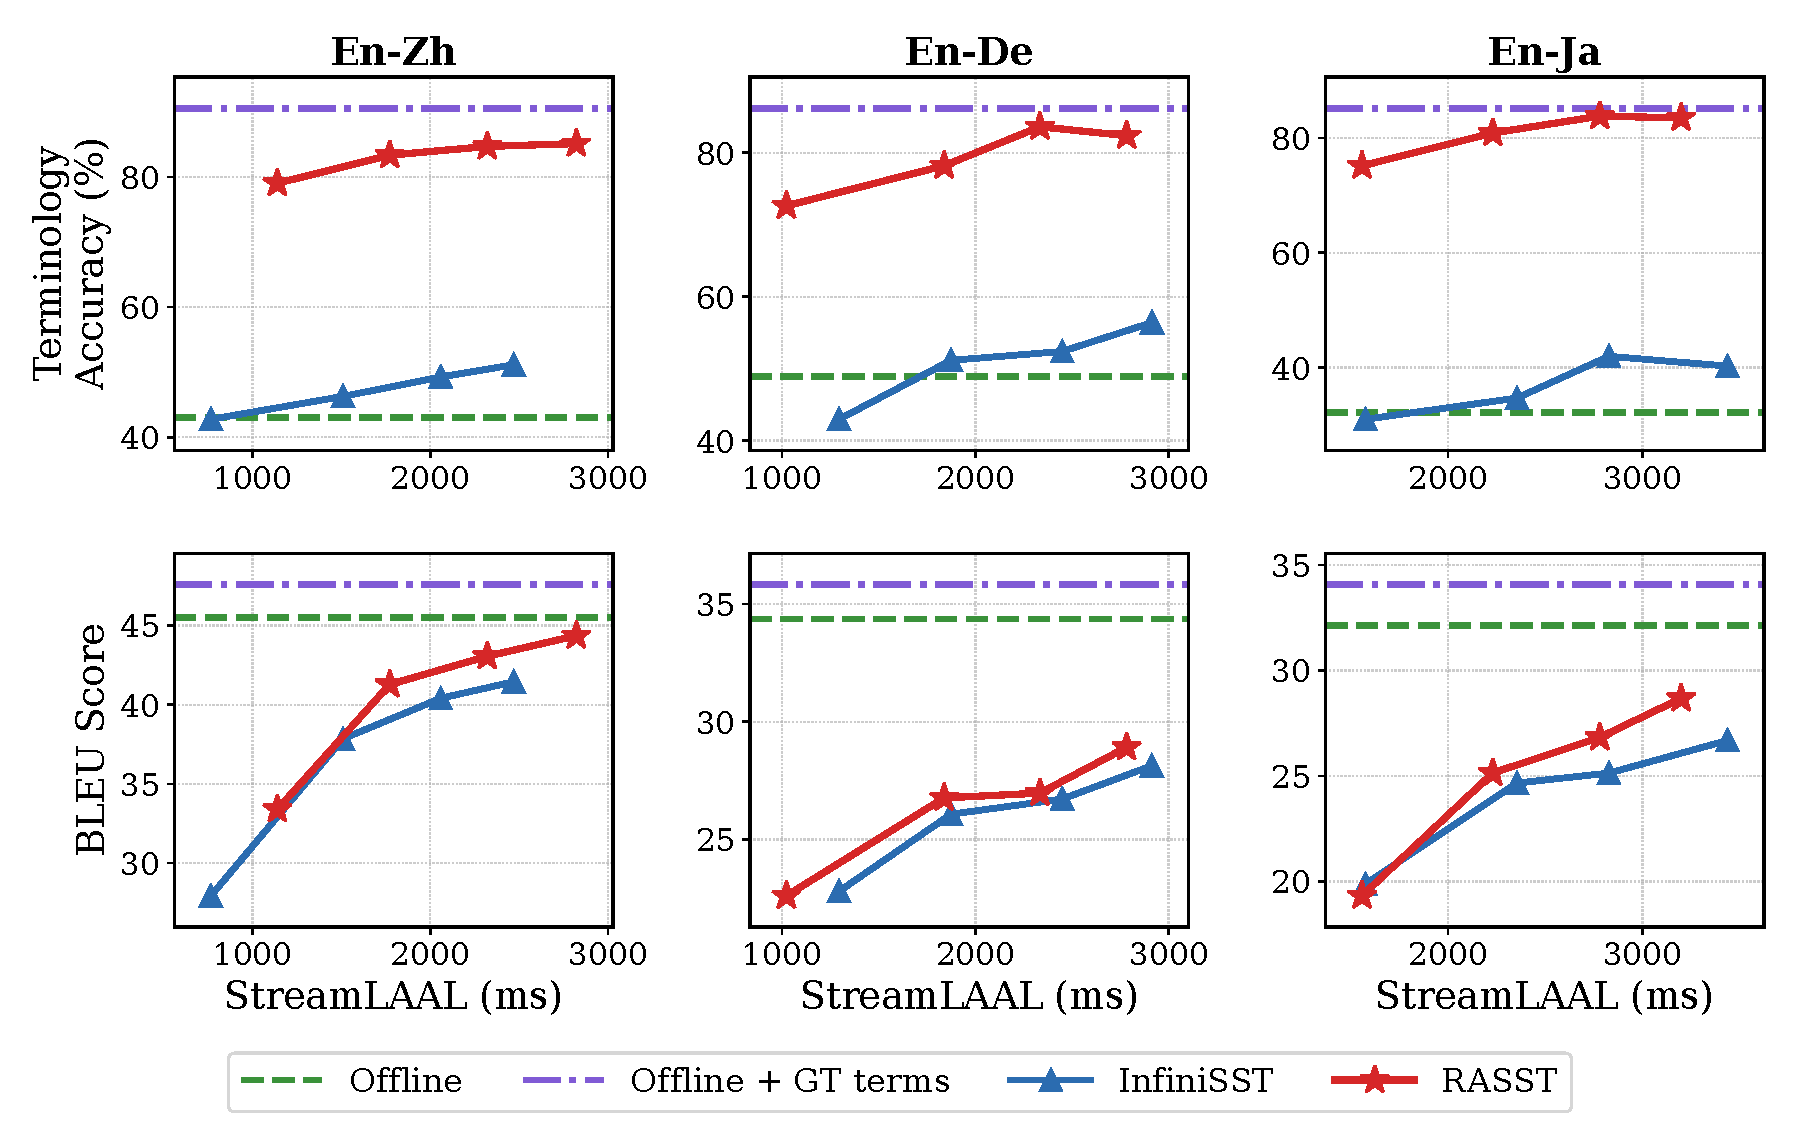
\includegraphics[width=0.9\linewidth]{latex/figures/medicine_main_result.pdf}
\caption{Main results on the manually curated medicine hardraw glossary. This is a strict domain stress test built from specialized clinical terms and exact target forms, rather than a broad easy glossary. We compare Terminology Accuracy (top) and BLEU (bottom) against StreamLAAL for En-Zh, En-De, and En-Ja. Horizontal lines show full-context offline LLM references, without and with oracle glossary terms.}
\label{fig:main_result_2}
\end{figure*}

\subsection{Main Results}

\paragraph{\method substantially improves terminology translation accuracy}
As shown in the first row of Figures~\ref{fig:main_result_1} and~\ref{fig:main_result_2}, \method consistently improves terminology translation accuracy over the strong InfiniSST baseline on the ACL tagged raw glossary and on the medicine hardraw readout. The horizontal offline references separate full-context decoding from full-context decoding with ground-truth glossary terms, showing the behavior of the same offline LLM when oracle terminology is supplied. The ACL tagged results cover En-Zh, En-De, and En-Ja under the fixed raw-glossary denominator, while the medicine hardraw panel is a manually curated hard-domain stress test whose denominator emphasizes specialized clinical terms and exact target forms that are difficult for a retrieval-free streaming system.

\paragraph{\method improves overall translation quality}
As shown in the second row of Figures~\ref{fig:main_result_1} and~\ref{fig:main_result_2}, \method also improves overall translation quality in the strongest ACL tagged and clean medicine En$\rightarrow$Zh comparisons. The BLEU gains are smaller than the terminology-accuracy gains, reflecting that specialized terms occur relatively infrequently in the speech and that the main effect of retrieval is concentrated on those terms.

\begin{figure}[t]
  \centering
  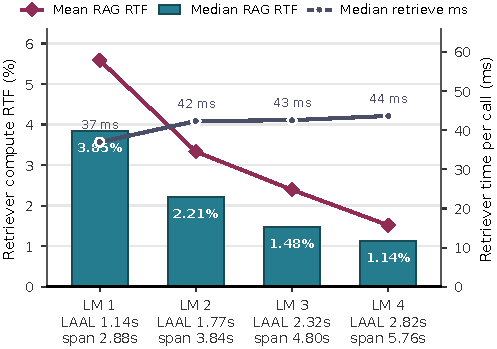
\includegraphics[width=\linewidth]{latex/figures/rag_compute_rtf.pdf}
  \caption{RAG compute real-time factor under timeline retrieval. We compute $\mathrm{RTF}_{\mathrm{RAG}} = t_{\mathrm{retrieve}} / (0.96\,\mathrm{s}\times\mathrm{LM})$ from verified En-Zh medicine hardraw runtime traces. The retriever runs once per vLLM generation step and encodes the current generation span plus a fixed $1.92\,\mathrm{s}$ look-back. Bars show median per-call RTF, the magenta line shows mean RTF, and the gray line shows median retriever time. Even as the encoded span grows from $2.88$ to $5.76$ seconds, the median RAG compute share falls from $3.85\%$ to $1.14\%$.}
  \label{fig:rag_compute_rtf}
\end{figure}

\paragraph{Computational efficiency}
Figure~\ref{fig:rag_compute_rtf} reports the retriever-side compute budget under the same timeline retrieval policy used by \method. Since retrieval is placed on a separate GPU and is invoked once per vLLM call, this is not additional user-visible StreamLAAL by itself; it measures how much retriever compute must fit inside each generation cadence interval. The median retrieval call stays around $37$--$44$ ms, and normalizing by the slower LM cadence makes the RAG compute share decrease as StreamLAAL increases.

\subsection{Ablation Studies}
\label{sec:ablations}

We group ablations by the component they test: retriever data and architecture, retriever calibration, Speech LLM term-map supervision, and online retrieval behavior. Unless otherwise stated, all terminology metrics use the same fixed raw-glossary denominator as the main results.

\begin{figure}[t]
\centering
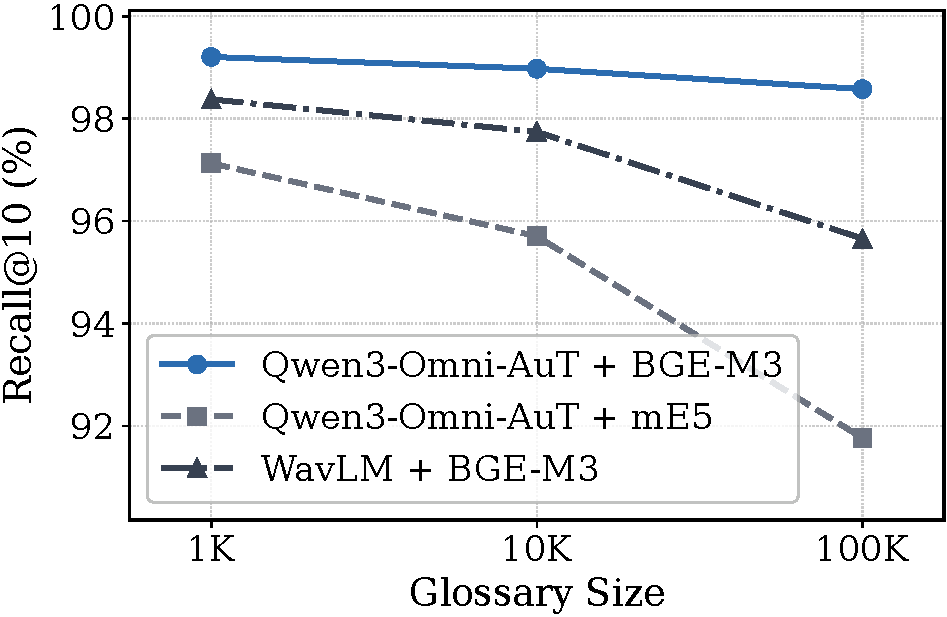
\includegraphics[width=\linewidth]{latex/figures/retriever_encoder_ablation_devraw.pdf}
\caption{Retriever encoder ablation on the development set. The Qwen3-Omni-AuT + BGE-M3 line is our main retriever encoder configuration. All points report Recall@10 with the denominator fixed to the dev raw glossary. Raw uses only the development glossary as the candidate bank, while GigaSpeech-10k and GigaSpeech-100k add 10k or 100k GigaSpeech-derived distractor terms to the runtime retrieval bank without changing the scoring denominator.}
\label{fig:ablation_retriever_encoder}
\end{figure}

\begin{figure}[t]
\centering
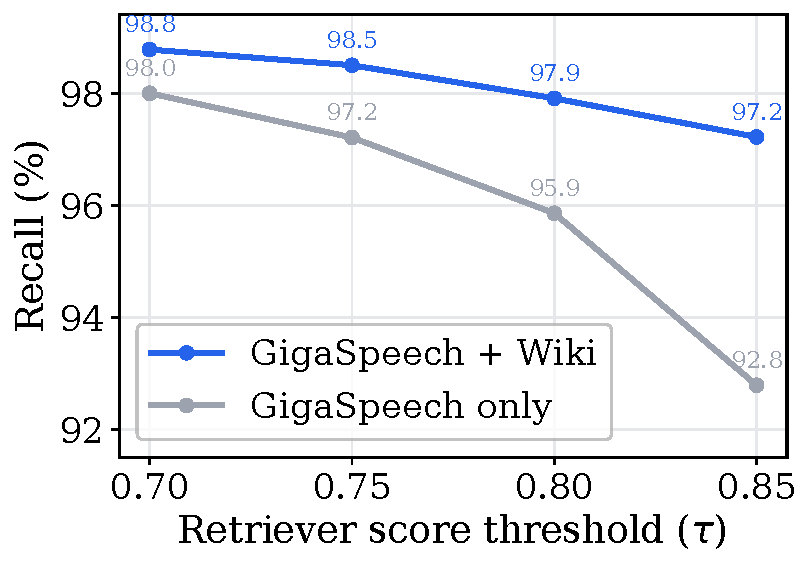
\includegraphics[width=\linewidth]{latex/figures/retriever_data_ablation_dev.pdf}
\caption{Retriever training-data ablation on the development set. The main retriever uses both GigaSpeech-derived supervision and Wiki-synthetic terminology examples, while the ablation removes the Wiki-synthetic rows and trains only on GigaSpeech. The left panel shows the checkpoint-selection metric, dev Recall@10 with a GS-10k retrieval bank. The right panel shows threshold-filtered dev recall with the same bank.}
\label{fig:ablation_retriever_data}
\end{figure}

\paragraph{Retriever training data}
Figure~\ref{fig:ablation_retriever_data} compares the main retriever against a GigaSpeech-only variant using the same development readout used for main retriever selection. Adding Wiki-synthetic terminology supervision improves dev Recall@10 with the GS-10k bank from 98.30 to 99.01. The difference is larger under stricter score filtering: at $\tau{=}0.80$, filtered dev recall increases from 95.86 to 97.91. This suggests that the synthetic text-derived terminology examples mainly improve robust retrieval under noisy or expanded runtime banks, rather than only increasing unfiltered top-k recall.

\begin{table}[t]
\centering
\small
\setlength{\tabcolsep}{4pt}
\begin{tabular}{lccc}
\toprule
Training context & Raw & GS-10k & GS-100k \\
\midrule
Fixed 1.92s & 98.11 & 97.47 & 95.18 \\
Fixed 3.84s & 98.65 & 98.31 & 97.58 \\
Fixed 5.76s & \textbf{99.64} & \textbf{99.58} & \textbf{99.33} \\
Variable 2.88--5.76s & 99.20 & 98.97 & 98.58 \\
\bottomrule
\end{tabular}
\caption{Retriever context-duration ablation on development data. Values are Recall@10 (\%) under fixed raw-denominator scoring. Raw uses only the per-context development glossary as the retrieval bank, while GS-10k and GS-100k add GigaSpeech-derived distractor terms to the runtime bank without changing the scoring denominator.}
\label{tab:ablation_context}
\end{table}

\paragraph{Retriever context construction}
Table~\ref{tab:ablation_context} compares fixed-context retrievers with the variable-context training used by \method. The fixed 5.76s setting is strongest because it always exposes the longest acoustic span. The variable-context retriever is within 0.44, 0.61, and 0.75 recall points of fixed 5.76s on the raw, GS-10k, and GS-100k banks, respectively, while matching the online contexts induced by latency multipliers 1--4 plus the fixed 1.92s look-back. We therefore use variable-context training in the main system: it retains most of the long-context retrieval benefit without assuming that every streaming step has a fixed 5.76s context.

\paragraph{Retriever encoders}
Figure~\ref{fig:ablation_retriever_encoder} tests whether the main Qwen3-Omni-AuT audio encoder and BGE-M3 dense text encoder are necessary. The GigaSpeech-expanded banks increase only the retrieval candidate set, so a robust encoder should preserve high recall even when many extra distractor terms are present. Replacing BGE-M3 with multilingual-E5 hurts robustness as the bank expands, while replacing Qwen3-Omni-AuT with WavLM has a smaller but consistent cost under the same fixed-denominator protocol.

\begin{figure*}[t]
\centering
% Dev-only tau-selection evidence: fixed raw denominator over raw/10k/100k banks.
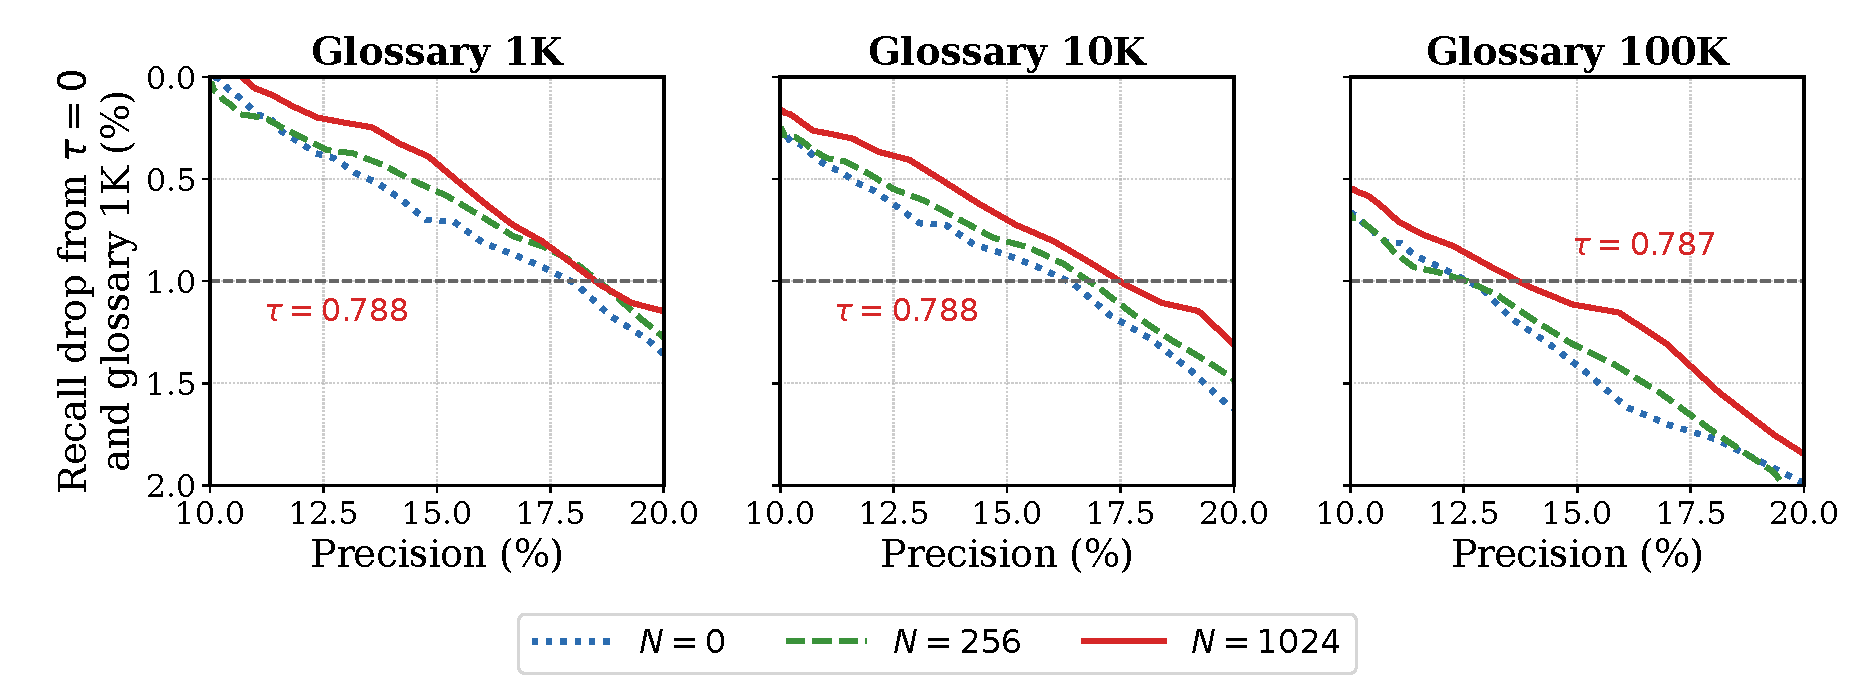
\includegraphics[width=0.9\linewidth]{latex/figures/retriever_dev_pr_fixedraw_hn_comparison.pdf}
\caption{Retriever hard-negative and threshold calibration ablation on development data. The figure reports fixed-raw-denominator precision-recall curves over multiple retrieval-bank sizes for no-HN, HN256, and HN1024. HN1024 is the main setting. The dashed vertical line marks the dev-only threshold-selection point where HN1024 recall drops by 1 percentage point from its raw-bank reference, yielding the operating region used by \method.}
\label{fig:ablation_hn_tau}
\end{figure*}

\paragraph{Hard negatives and threshold sweep}
Figure~\ref{fig:ablation_hn_tau} shows the available development-only evidence for hard-negative training and threshold selection. We use the fixed raw-glossary denominator when sweeping $\tau$ so that larger retrieval banks affect only the retrieved candidates, not the evaluation scope. HN1024 gives the strongest precision-recall tradeoff among the available curves. The dashed line indicates the recall-preserving operating point: the largest threshold before the HN1024 curve has lost 1 percentage point of recall relative to its raw-bank reference, which places the selected deployment threshold near $\tau{=}0.78$.

\begin{figure*}[t]
\centering
\includegraphics[width=0.9\linewidth]{latex/figures/speechllm_ablation_de.pdf}
\caption{Speech LLM ablation on En-De ACL tagged evaluation. We reuse the En-De rows from the earlier tagged main-result figure, rename its old \method line as \textit{RASST (LLM-generated TM SFT)}, and add the current \method En-De result from Figure~\ref{fig:main_result_1}. The blue horizontal line is the full-context offline LLM upper bound with oracle glossary terms.}
\label{fig:ablation_speechllm}
\end{figure*}

\paragraph{Speech LLM term-map supervision}
Figure~\ref{fig:ablation_speechllm} isolates the Speech LLM term-map supervision effect on En-De. The no-TM-SFT system uses runtime RAG without term-map supervision, while the historical LLM-generated TM-SFT line trains the Speech LLM on dense LLM-generated term maps. The current \method line replaces those dense LLM-generated maps with the retriever-style term maps used in the main system, improving terminology accuracy while moving toward the oracle-term upper bound.

\begin{figure}[t]
\centering
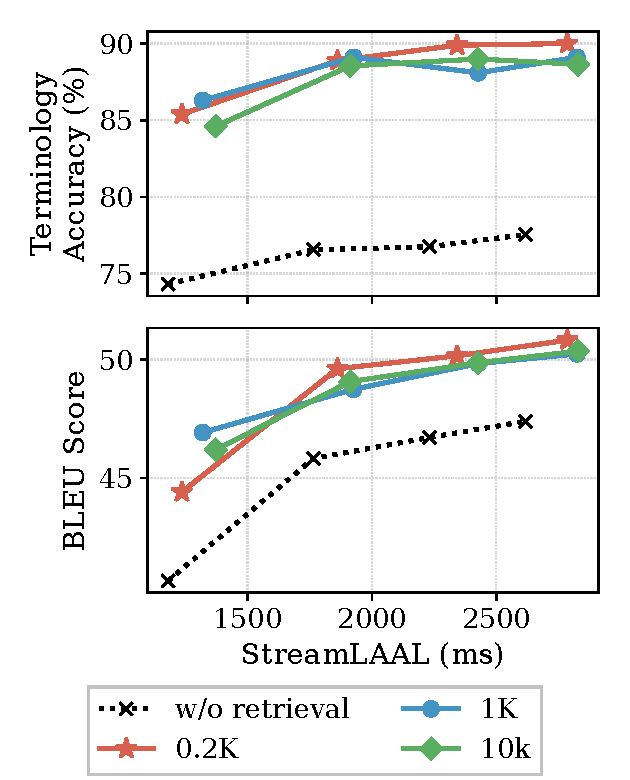
\includegraphics[width=\linewidth]{latex/figures/glossary_bank_ablation_zh_fixedraw.pdf}
\caption{Runtime glossary-bank ablation on the En-Zh ACL tagged evaluation. The runtime retrieval bank changes from the raw tagged glossary to GS-1k and GS-10k expanded banks, while terminology metrics are always scored against the fixed raw tagged denominator. Points are ordered by latency multiplier from 1 to 4.}
\label{fig:ablation_glossary_bank}
\end{figure}

\paragraph{Runtime glossary-bank expansion}
Figure~\ref{fig:ablation_glossary_bank} tests whether \method remains stable as the runtime terminology bank grows. The evaluation denominator is fixed to the raw tagged glossary, so changes in TERM\_ACC reflect retrieval and generation behavior under additional distractor terms rather than a changing metric scope. Expanding to GS-1k and GS-10k preserves BLEU and keeps TERM\_ACC close to the raw-bank setting across latency multipliers, while FCR remains controlled. This shows that the system remains usable with larger runtime banks, though the appendix stress test shows that bank quality and duplicate control still matter. Full ACL rows and the stricter medicine stress-test rows are reported in Appendix~\ref{app:glossary_bank_ablation}.

\begin{figure}[t]
\centering
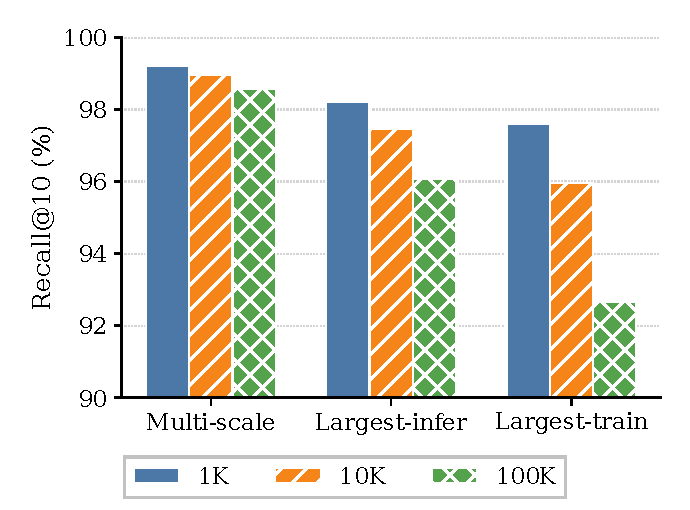
\includegraphics[width=\linewidth]{latex/figures/multiscale_inference_ablation_devraw.pdf}
\caption{Multi-scale inference ablation on development data. The first two systems reuse the same MFA-supervised variable-context retriever and fixed raw-denominator scoring; only the runtime MaxSim window set changes from all windows to the largest internal window. The dense 1.92s system is the historical single-embedding retriever trained without MFA window localization. Expanded banks add GigaSpeech distractors only at retrieval time.}
\label{fig:ablation_multiscale_inference}
\end{figure}

\paragraph{MaxSim inference}
Figure~\ref{fig:ablation_multiscale_inference} examines the contribution of multi-scale inference. The main retriever scores candidate terms with MaxSim over speech-window embeddings, allowing short terminology mentions to match the most relevant part of the current speech context. Reusing the same retriever but querying only the largest internal window lowers dev Recall@10 on the GS-100k bank from 98.58 to 96.07, and lowers filtered recall at $\tau{=}0.75$ from 98.42 to 93.62. This shows that the smaller windows are not redundant at inference time. We also compare against a historical dense 1.92s retriever trained directly as a single audio embedding, which removes the MFA-window training--inference mismatch but underperforms on the expanded bank, reaching 92.65 Recall@10 and only 23.94 filtered recall at $\tau{=}0.75$. The result indicates that dense one-shot speech embeddings have much weaker score calibration for thresholded retrieval than the multi-scale MaxSim formulation.

\paragraph{Real-time factor}
The RAG compute-RTF readout in Figure~\ref{fig:rag_compute_rtf} is reported separately from quality ablations because it measures runtime budget rather than retrieval accuracy. End-to-end latency is still represented by StreamLAAL in the main result curves.

\clearpage
